\section{Paradigms}

There exist a broad set of theoretical paradigms for explaining the role of consciousness in terms of functional characteristics and their attributed survival advantage, its relation to physical laws of nature, and the phenomenal conscious experience -- \textit{``the ghost in the shell.''}

\subsection{Information Integration Theory}

Christof Koch et al. \cite{foo} place consciousness on a gradient from minimal consciousness to more complex states of consciousness (an entity can be more or less conscious), and proclaim that consciousness can arise in any organism or artificial system which exhibit sufficient integration of information (such as combining information from different sensory modalities). This theoretical paradigm is referred to as Information Integration Theory (IIT) and has paved way for research on the Neural Correlates of Consciousness (NCC), the minimal set of neural activity correlated with states of consciousness.

In this view, anaesthesia as used during surgery could temporarily inhibit or limit the information integration capacity of the brain, such that the patient would fall unconscious (or reach a minimal state of consciousness).

The moral implications of IIT if fully considered are substantial, both with regards to diagnosis of patient in coma and vegitative states (\todo{find politically correct word for vegitative}), but also for non-biological entities; as realised when reflecting on the following quote by Christof Koch (\todo{add cite to Christof Koch - Can Consciousness be Non-Biological-XG-hpuhbSyo}).

\begin{quote}
	\textit{``The Internet as a whole potentially has some conscious state. I don't think you can rule it out today categorically.''}
\end{quote}

\subsection{Bayesian Predictive Coding}

% We should have anticipations about everything that matters to us.

%From as early as the 19th century, it has been hypothesized

\begin{figure}[htbp]
	\begin{center}
		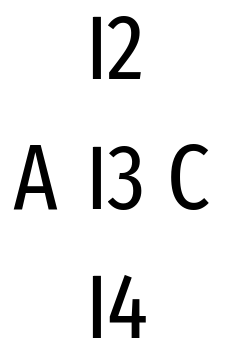
\includegraphics[width=0.3\textwidth]{inc/abc.png}
		\caption{Read from left-to-right primes for \textit{``B''} while reading top-to-bottom primes for \textit{``13''}.}
		\label{fig:abc}
	\end{center}
\end{figure}

\todo{foo} \cite{predictive_coding}

\subsection{Emergent Phenomena}

\todo{foo}

\subsection{foo}

\todo{foo}
